\documentclass[12pt]{report}
\usepackage[utf8]{inputenc}
\usepackage[russian]{babel}
%\usepackage[14pt]{extsizes}
\usepackage{listings}

% Для листинга кода:
\usepackage{indentfirst}
\usepackage{titlesec, blindtext, color} 
\definecolor{gray75}{gray}{0.75} 
\newcommand{\hsp}{\hspace{20pt}}
\usepackage{color} %% это для отображения цвета в коде
\usepackage{caption}
\DeclareCaptionFormat{listing}{\colorbox{gray}{\parbox{\textwidth}{#1#2#3}}}
\titleformat{\chapter}[hang]{\Huge\bfseries}{\thechapter\hsp\textcolor{gray75}{|}\hsp}{0pt}{\Huge\bfseries}

\usepackage{pdfpages}
\usepackage{titlesec}
\usepackage{pgfplots}
\usepackage{filecontents}
\usetikzlibrary{datavisualization}
\usetikzlibrary{datavisualization.formats.functions}
\setlength{\parindent}{5ex}
\setlength{\parskip}{1em}
\begin{filecontents}{LevR.dat}
0 0
7 0.05953125
8  0.31359387 
9 1.70062500 
10 9.67343751
11 53.6781259 
\end{filecontents}

\begin{filecontents}{LevT.dat}
0 0
7 0.00011573
8 0.00015625
9 0.00031250
10 0.00043863
11 0.00051859
\end{filecontents}

\begin{filecontents}{DamLevR.dat}
0 0
7 0.06006258 
8 0.34478142 
9 1.88374617 
10 11.82792422 
11 56.38492565
\end{filecontents}

\begin{filecontents}{DamLevT.dat}
0 0
7 0.0001696
8 0.00029921
9 0.00033949
10 0.00483723
11 0.00054846
\end{filecontents}


\begin{document}
\lstset{ %
language=Python,                 % выбор языка для подсветки (здесь это С)
basicstyle=\small\sffamily, % размер и начертание шрифта для подсветки кода
numberstyle=\tiny,           % размер шрифта для номеров строк
stepnumber=1,                   % размер шага между двумя номерами строк
numbersep=3pt,                % как далеко отстоят номера строк от подсвечиваемого кода
backgroundcolor=\color{white}, % цвет фона подсветки - используем \usepackage{color}
showspaces=false,            % показывать или нет пробелы специальными отступами
showstringspaces=false,      % показывать или нет пробелы в строках
showtabs=false,             % показывать или нет табуляцию в строках
frame=single,              % рисовать рамку вокруг кода
tabsize=2,                 % размер табуляции по умолчанию равен 2 пробелам
captionpos=t,              % позиция заголовка вверху [t] или внизу [b] 
breaklines=true,           % автоматически переносить строки (да\нет)
breakatwhitespace=false, % переносить строки только если есть пробел
escapeinside={\%*}{*)},   % если нужно добавить комментарии в коде
}
%\def\chaptername{} % убирает "Глава"
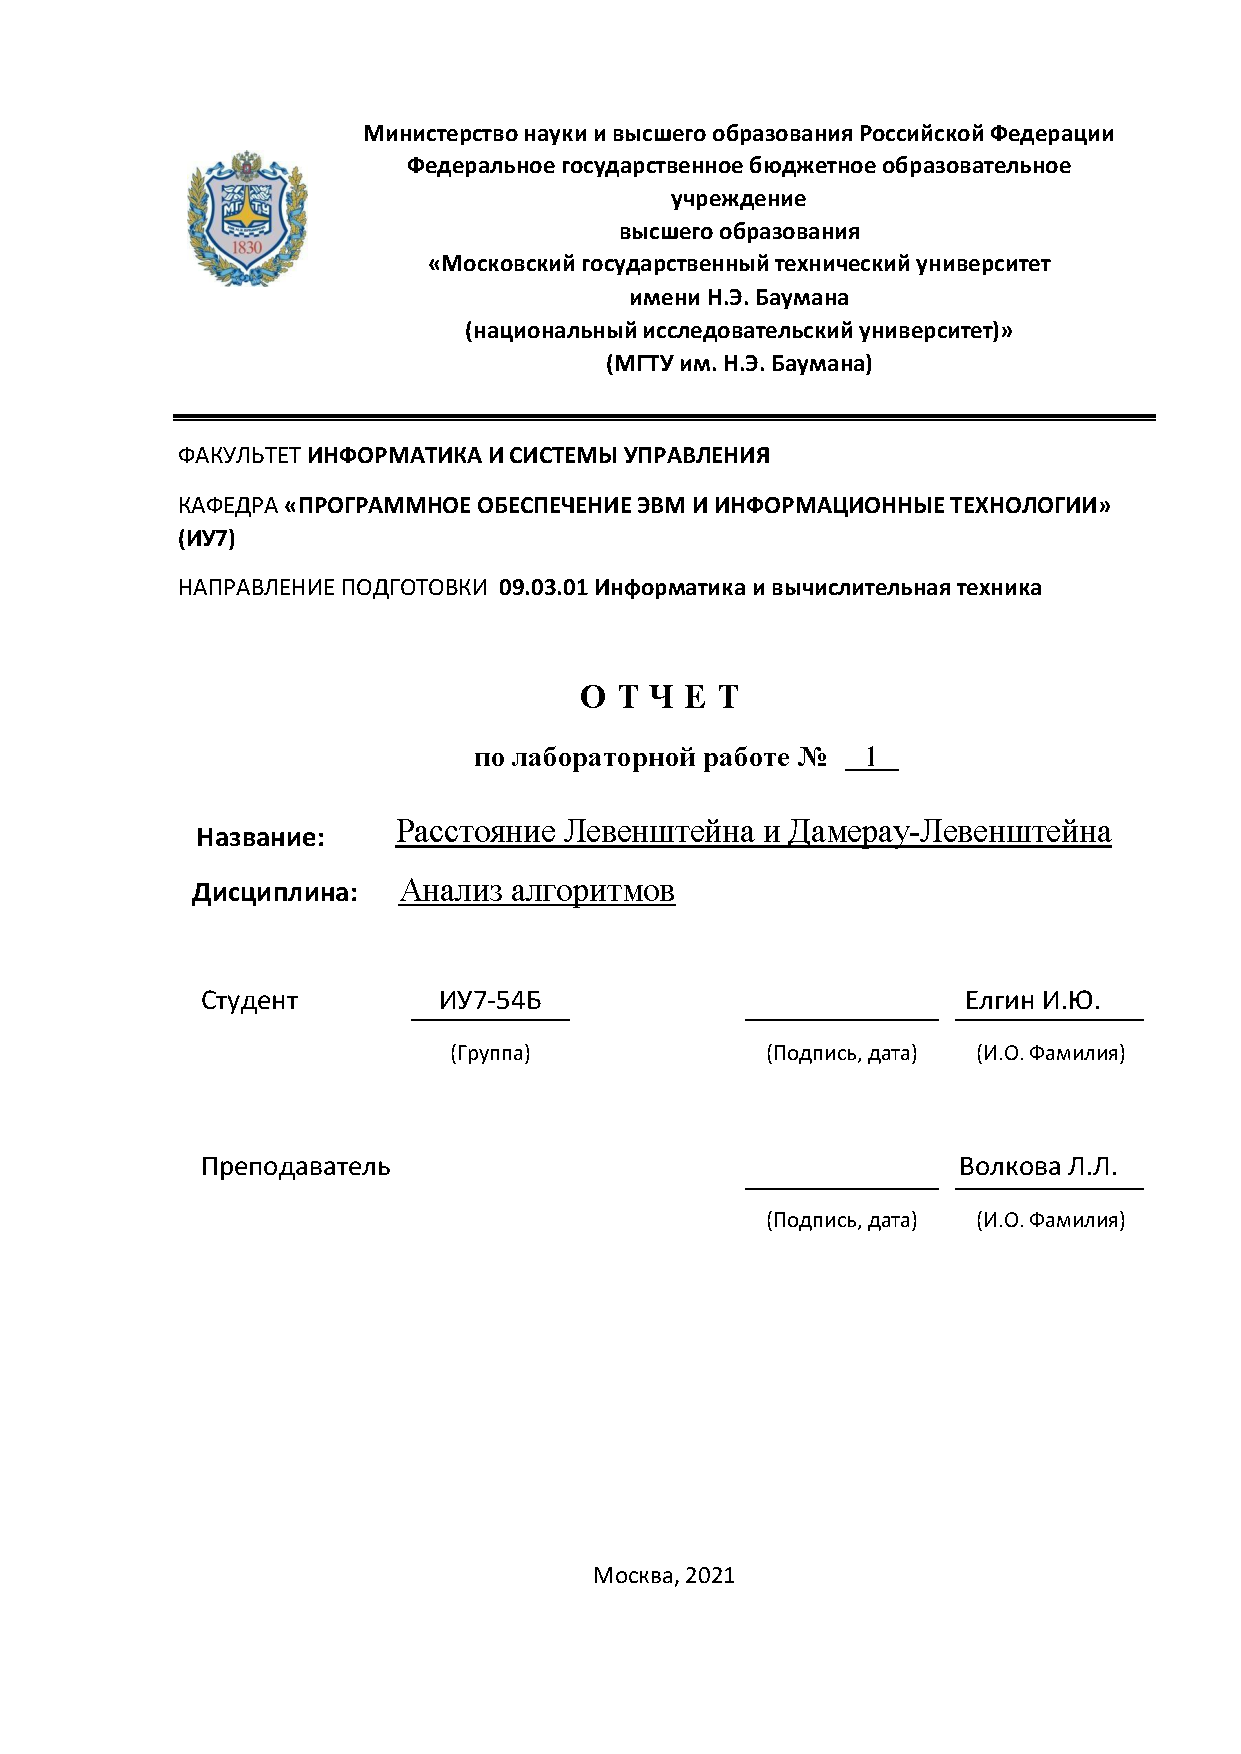
\includepdf[pages=1]{titul.pdf}

\tableofcontents

\newpage
\chapter*{Введение}
\addcontentsline{toc}{chapter}{Введение}
\textbf{Расстояние Левенштейна} - минимальное количество операций вставки одного символа, удаления одного символа и замены одного символа на другой, необходимых для превращения одной строки в другую \cite{declaration}.

Расстояние Левенштейна применяется в теории информации и компьютерной лингвистике для:

\begin{itemize}
	\item исправления ошибок в слове;
	\item сравнения текстовых файлов;
	\item в биоинформатике для сравнения генов, хромосом и белков.
\end{itemize}

Целью данной лабораторной работы является изучение метода динамического программирования на материале алгоритмов
Левенштейна и Дамерау-Левенштейна. 

Задачами данной лабораторной являются:
\begin{enumerate}
  	\item Изучение рекурсивных и нерекурсивных алгоритмов Левенштейна и Дамерау-Левенштейна нахождения расстояния между строками;
	\item Применение метода динамического программирования для нерекурсивной реализации алгоритмов Левенштейна и Дамерау-Левенштейна; 
	\item Получение практических навыков реализации следующих алгоритмов: алгоритм Левенштейна с кешом в две строки,алгоритм Дамерау-Левенштейна с матрицей, рекурсивный алгоритм Левенштейна, рекурсивный алгоритм Дамерау-Левенштейна; 
	\item Сравнительный анализ линейной и рекурсивной реализаций выбранного алгоритма определения расстояния между строками по затрачиваемым ресурсам (времени и памяти); 
	\item Экспериментальное подтверждение различий во временнóй эффективности рекурсивной и
нерекурсивной реализаций выбранного алгоритма; 
	\item Описание и обоснование полученных результатов в отчете о выполненной лабораторной
работе, выполненного как расчётно-пояснительная записка к работе. 
\end{enumerate}


\chapter{Аналитическая часть}
Задача по нахождению расстояния Левенштейна заключается в поиске минимального количества операций вставки/удаления/замены для превращения одной строки в другую.

При нахождении расстояния Дамерау — Левенштейна добавляется операция транспозиции (перестановки соседних символов).  
 
\textbf{Действия обозначаются так:} 
\begin{enumerate}
  	\item D (англ. delete) — удалить;
	\item I (англ. insert) — вставить;
	\item R (replace) — заменить;
	\item M (match) - совпадение;
	\item T (transposition) - транспозиция в алгоритме Дамерау - Левенштейна.
\end{enumerate}
\section{Анализ алгоритмов}
Пусть $S_{1}$ и $S_{2}$ — две строки (длиной M и N соответственно) над некоторым алфавитом, тогда расстояние Левенштейна можно подсчитать по следующей рекуррентной формуле:

\begin{displaymath}
D(i,j) = \left\{ \begin{array}{ll}
 0, & \textrm{$i = 0, j = 0$}\\
 i, & \textrm{$j = 0, i > 0$}\\
 j, & \textrm{$i = 0, j > 0$}\\
min(\\
D(i,j-1)+1,\\
D(i-1, j) +1, &\textrm{$j>0, i>0$}\\
D(i-1, j-1) + m(S_{1}[i], S_{2}[j])\\
),
  \end{array} \right.
\end{displaymath}

где $m(a,b)$ равна нулю, если $a=b$ и единице в противном случае; $min\{\,a,b,c\}$ возвращает наименьший из аргументов.

Расстояние Дамерау-Левенштейна вычисляется по следующей рекуррентной формуле:
\begin{displaymath}
D(i,j) = \left\{ \begin{array}{ll}
 0, & \textrm{$i = 0, j = 0$}\\
 i, & \textrm{$j = 0, i > 0$}\\
 j, & \textrm{$i = 0, j > 0$}\\
min(\\
D(i,j-1)+1,\\
D(i-1, j) +1, &\textrm{$j>0, i>0$}\\
D(i-1, j-1) + m(S_{1}[i], S_{2}[j])\\
D(i-2, j-2) + 1, &\textrm{if $i,j>1$ and $a_{i} = b_{j-1},a_{i-1}=b_{j} $}\\
).
  \end{array} \right.
\end{displaymath}

\section{Способ измерения времени работы алгоритма}
Существует два подхода для замера времени измерение реалного времени и измерение процессорного времени.

Измерение реального времени данный способ прост так как использует только разность системного времени начала и конца выполнения алгоритма. Однако процессы происходящие паралельно с выполнением алгоритма могут повлиять на скорость выполнения алгоритма в связи с чем реалное время работы алгоритма могут меняться.

Измерение процессорного времени замеряет время выполнения только процесса замеряемого алгоритма что даёт наиболее точный результат с меньшим количеством погрешностей вызваных другими процессами выполняющимися паралельно с данным.
Второй метод наиболее точен, поэтому выберем его.


\chapter{Конструкторская часть}
В данной главе рассматриваются требования к программе и приводятся схемы алгоритмов.
\section{Требования}
\textbf{Требования к вводу:}
\begin{enumerate}
  	\item На вход подаются две строки;
	\item Буквы верхнего и нижнего регистров считаются разными.
\end{enumerate}
\textbf{Требования к выводу:}
  	На выходе необходимо получить число означающее минимальное количество операций, необходимых для получения из одной строки другую. 
\newline	
\newline	
\textbf{Требования к программе:}
  	Программа должна коректно работать при вводе любых двух строк.
\section{Схемы алгоритмов}
На рисунках 2.1, 2.2, 2.3, 2.4, 2.5, 2.6 приведены схемы рекурсивных и нерекурсивных алгоритмов Левенштейна и Дамерау ливенштейна.
\begin{figure}[h!]
\center{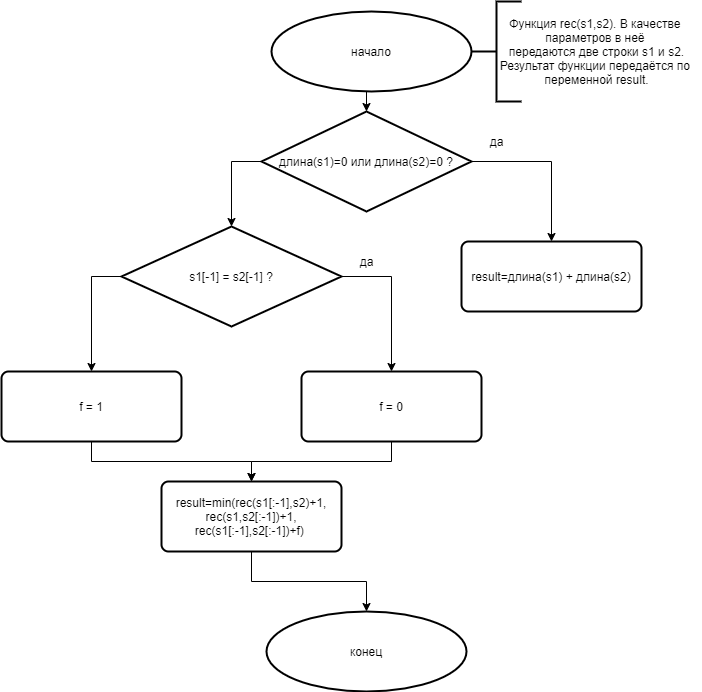
\includegraphics[scale=0.7]{levenshtainrec.png}}
\caption{Рекурсивный алгоритм Левенштейна}
\end{figure}
\begin{figure}[h!]
\center{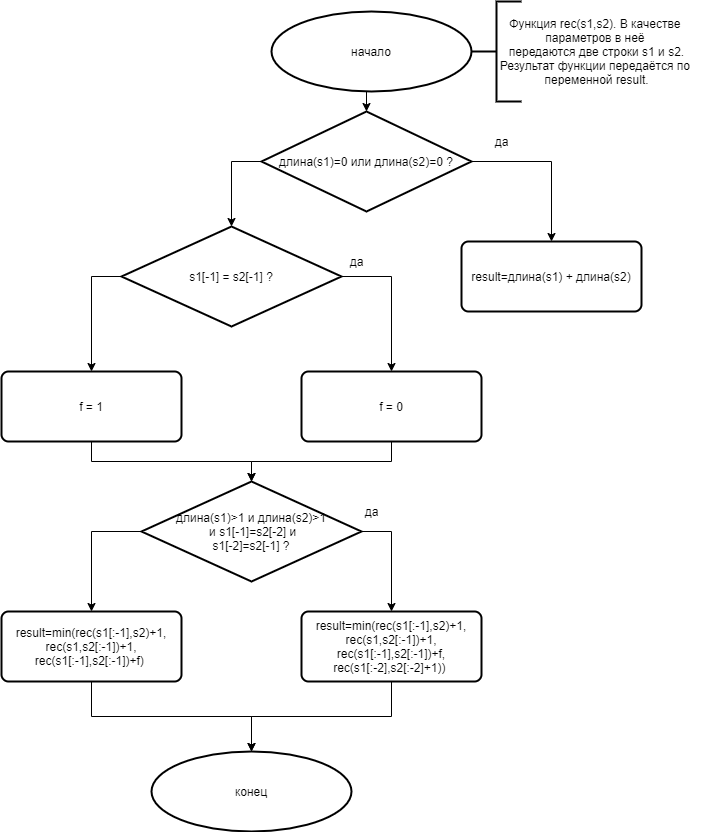
\includegraphics[scale=0.7]{dameraurec.png}}
\caption{Рекурсивный алгоритм Дамерау-Левенштейна}
\end{figure}
\begin{figure}[h!]
\center{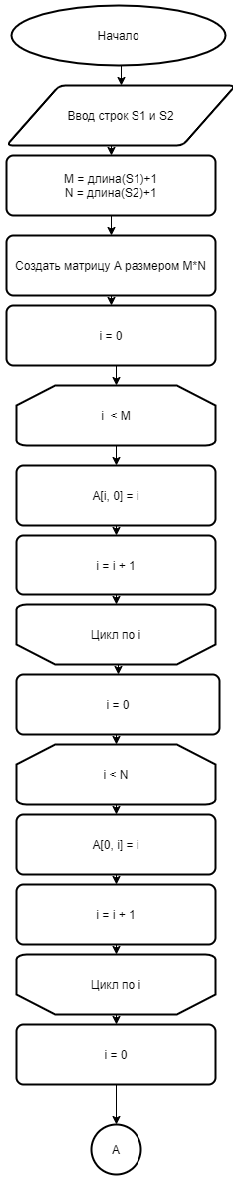
\includegraphics[scale=0.6]{levenshtain2str.png}}
\caption{Алгоритм Левенштейна с кэшем в две строки часть 1}
\end{figure}
\begin{figure}[h!]
\center{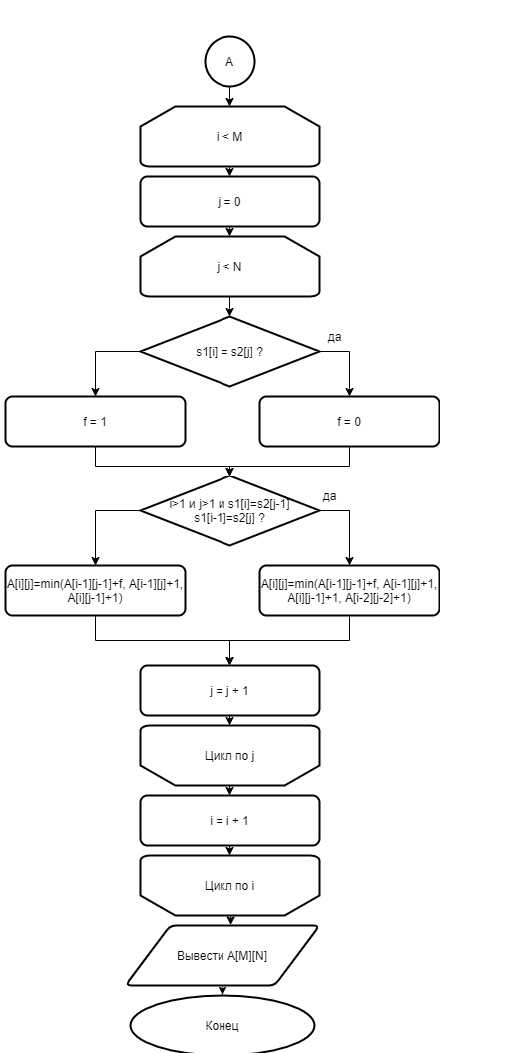
\includegraphics[scale=0.6]{levenshtain2str2.png}}
\caption{Алгоритм Левенштейна с кэшем в две строки часть 2}
\end{figure}
\begin{figure}[h!]
\center{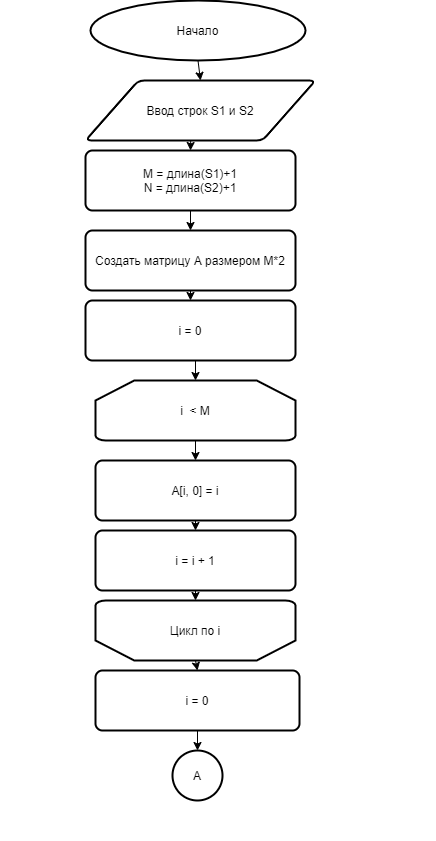
\includegraphics[scale=0.8]{damerautable.png}}
\caption{Алгоритм Дамерау-Левенштейна с кэшем в виде матрицы часть 1}
\end{figure}
\begin{figure}[h!]
\center{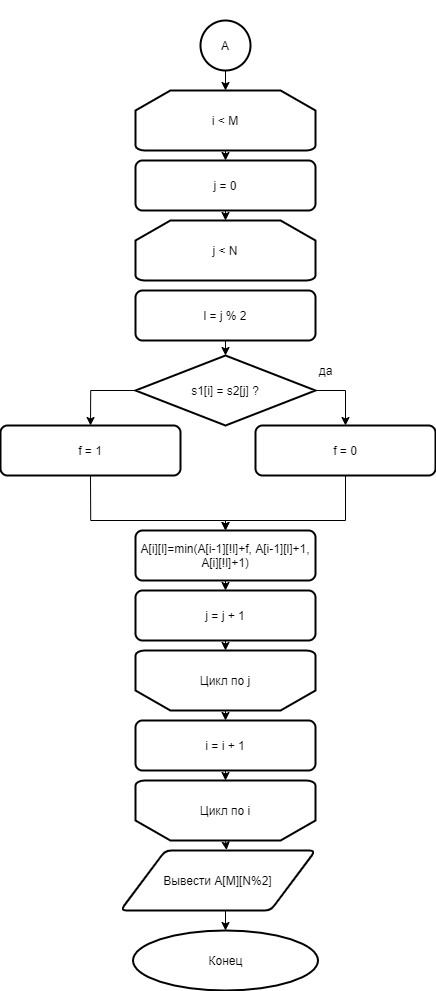
\includegraphics[scale=0.7]{damerautable2.png}}
\caption{Алгоритм Дамерау-Левенштейна с кэшем в виде матрицы часть 2}
\end{figure}
\chapter{Технологическая часть}
В данной главе выбирается язык программирования для реализации рекурсивных и нерекурсивные алгоритмы Левенштейна и Дамерау-Левенштейна, приводятся листинги функций реализующих данные алгоритмы. Приводится тестирование данных алгоритмов и сравнение памяти используемой алгоритмами.
\section{Выбор ЯП}
В качестве языком программирования мною выбран язык Python, так как я имею опыт работы с данным языком программирования, Pyton позволяет удобно работать со строками и матрицами.

Время работы алгоритмов было замерено с помощью функции process\_time() из библиотеки time \cite{lit}.

\section{Сведения о модулях программы}
Программа состоит из:
\begin{itemize}
	\item lab1.py - главный файл программы, в котором располагаются алгоритмы, меню и тесты
\end{itemize}

\begin{lstlisting}[label=some-code,caption=Функция нахождения расстояния Левенштейна рекурсивно]
def levensteinRecursion(s1, s2):
    if (s1 == "" or s2 == ""):
        return len(s1) + len(s2)

    if (s1[-1] == s2[-1]): 
        f = 0 
    else: 
        f = 1

    return min(levensteinRecursion(s1[:-1], s2) + 1,
               levensteinRecursion(s1, s2[:-1]) + 1,
               levensteinRecursion(s1[:-1], s2[:-1]) + f)
\end{lstlisting}

\begin{lstlisting}[label=some-code,caption=Функция нахождения расстояния Левенштейна с кешом в 2 строки]
def levensteinTable(s1, s2, isPrint):
    lenI = len(s1) + 1
    lenJ = len(s2) + 1

    table = [[j for j in range(lenJ)] for i in range(2)]
    for i in range(1, lenI):
        for j in range(1, lenJ):
            l = i % 2
            table[l][0] = i
            if (s1[i - 1] == s2[j - 1]):
                f = 0 
            else:
                f = 1
            table[l][j] = min(table[not l][j] + 1,
                              table[l][j-1] + 1,
                              table[not l][j - 1] + f)
            
    return table[-1][-1]
\end{lstlisting}

\begin{lstlisting}[label=some-code,caption=Функция нахождения расстояния Дамерау-Левенштейна рекурсивно]
def DameraulevensteinRecursion(s1, s2):
    if (s1 == "" or s2 == ""):
        return len(s1) + len(s2)

    if (s1[-1] == s2[-1]): 
        f = 0 
    else: 
        f = 1
    if (len(s1) > 1 and len(s2) > 1 and s1[-2] == s2[-1] and s1[-1] == s2[-2]):
        return min(DameraulevensteinRecursion(s1[:-1], s2) + 1,
               DameraulevensteinRecursion(s1, s2[:-1]) + 1,
               DameraulevensteinRecursion(s1[:-1], s2[:-1]) + f,
                DameraulevensteinRecursion(s1[:-2], s2[:-2]) + 1)
    else:
        return min(DameraulevensteinRecursion(s1[:-1], s2) + 1,
               DameraulevensteinRecursion(s1, s2[:-1]) + 1,
               DameraulevensteinRecursion(s1[:-1], s2[:-1]) + f)
\end{lstlisting}

\begin{lstlisting}[label=some-code,caption=Функция нахождения расстояния Дамерау-Левенштейна матрично]
def damerauLevenstein(s1, s2, isPrint):
    lenI = len(s1) + 1
    lenJ = len(s2) + 1
    
    table = [[i + j for j in range(lenJ)] for i in range(lenI)]

    for i in range(1, lenI):
        for j in range(1, lenJ):
            if (s1[i - 1] == s2[j - 1]):
                f = 0
            else:
                f = 1
            
            table[i][j] = min(table[i - 1][j] + 1,
                              table[i][j - 1] + 1,
                              table[i - 1][j - 1] + f)
            
            if (i > 1 and j > 1 and s1[i - 1] == s2[j - 2] and s1[i - 2] == s2[j - 1]):
                table[i][j] = min(table[i][j], table[i - 2][j - 2] + 1)

    if isPrint:
        tablePrint(table)
    
    return table[-1][-1]
\end{lstlisting}

\section{Тесты}
Было организовано функциональное тестирование по принципу чёрного ящика.

Тестирование проводилось на подготовленных данных, наборы тестовых случаев полностью покрывают функциональную область. Данные тестов приведены в таблице 3.1.

\begin{table}[h!]
	\begin{tabular}{|c|c|c|c|c|c|c|} 
 	\hline
	test & str1 & str2 & Lev Rec & Dam Rec & Lev 2 str & Dam Tab \\ [0.5ex] 
 	\hline\hline
 	пустой & "" & "" & 0 & 0 & 0 & 0\\
 	\hline
 	пустой & "" & "f" & 1 & 1 & 1 & 1\\
 	\hline
	пустой & "f" & "" & 1 & 1 & 1 & 1\\
	\hline
	совпадающий & "asd" & "asd" & 0 & 0 & 0 & 0\\
 	\hline
 	совпадающий & "f" & "f" & 0 & 0 & 0 & 0\\
 	\hline
	совпадающий & "f" & "F" & 1 & 1 & 1 & 1\\
	\hline
	случайный & "a" & "s" & 1 & 1 & 1 & 1\\
 	\hline
 	случайный & "asd" & "bsf" & 2 & 2 & 2 & 2\\
 	\hline
	случайный & "asd" & "as" & 1 & 1 & 1 & 1\\
	\hline
 	случайный & "a" & "adws" & 3 & 3 & 3 & 3\\
 	\hline
 	случайный & "as" & "sa" & 2 & 1 & 2 & 1\\
 	\hline
	\hline
	\end{tabular}
\caption{Тестовые случаи с данными и результатами}
\end{table}

Для тестирования функций по времени создаётся случайная строка, заданной длины.

\begin{lstlisting}[label=takeRandomString,caption=Функция генерации случайной строки]
def takeRandomString(size):
    return ''.join(random.choice(string.ascii_letters) for _ in range(size))
\end{lstlisting}

\section{Сравнительный анализ алгоритмов по памяти}
Пусть на вход подаются строки длинами \textit{m} и \textit{n}. Учитывая специфику реализации, можно получить формулу вычисления памяти в байтах;
\newline

\begin{equation}X_{matr} = ((m+1)*(n+1))*Sizeof(int) 
\end{equation}
\newline
\newline
Также в алгоритме используется 2 переменных под размеры \textit{n} и \textit{m}, 2 под циклы, сами строки \textit{m} и \textit{n} и 1 переменная под флаг.
\newline
Итоговый размер в байтах \begin{equation}X_{matr} = 4((m+1)*(n+1)) + m + n + 20 
\end{equation}
\newline
\newline
\begin{equation}
2*S_{string} = 2*m*Sizeof(int)  
\end{equation}
\newline
\newline
Также в алгоритме используется 2 переменных под размеры \textit{n} и \textit{m}, 2 под циклы, сами строки \textit{m} и \textit{n} и 2 переменных под флаг.
\newline
Итоговый размер в байтах \begin{equation}2*S_{string} = 8*(m+1) + m + n + 24 
\end{equation}
\newline
\newline
В рекурсивных алгоритмах количество занимаемой памяти зависит от глубины рекурсии. Глубина рекурсии равна \textit{m+n}. Количество дополнительных переменных в рекурсивных алгоритмах Левенштейна и Дамерау-Левенштейна совпадают, поэтому памяти на них будет выделено одинаково.

\begin{equation}X_{recur} = \sum_{i=0}^{m+n} (2*S_{string}+(m+n+2-i)*S_{char}+c*S_i) \end{equation}

Результаты подсчёта памяти в байтах для приведённых выше алгоритмов для различных размеров строк приведены в таблице 3.2.
\newline
\begin{table}[h!]
	\begin{tabular}{|c|c|c|c|c|} 
 	\hline
	str len & Levenshtain Rec & Damamerau Rec & Levenshtain 2 str & Damerau Tab \\ [0.5ex] 
 	\hline\hline
 	10 & 1270 & 1270 & 132 & 524\\
 	\hline
 	50 & 10350 & 10350 & 532 & 10524\\
 	\hline
	100 & 30700 & 30700 & 1032 & 41024\\
	\hline
	500 & 553500 & 553500 & 5032 & 1005024\\
	\hline
	\end{tabular}
\caption{Сравнение памяти, потребляемой алгоритмами}
\end{table}

\chapter{Исследовательская часть}
В данной главе исследуются временные показатели для рекурсивных и нерекурсивных алгортитмов Левенштейна и Дамерау-Левенштейна.
\section{Результаты временных тестов} 
Был проведен замер времени работы каждого из алгоритмов. Результаты замеров в секундах приведены в таблице 4.1.
\begin{table}[h!]
	\begin{tabular}{|c|c|c|c|c|} 
 	\hline
	str len & Levenshtain Rec & Damamerau Rec & Levenshtain 2 str & Damerau Tab \\ [0.5ex] 
 	\hline\hline
 	7 & 0.05953125 & 0.06006258 & 0.00011573 & 0.0001696\\
 	\hline
 	8 & 0.31359387 & 0.34478142 & 0.00015625 & 0.00029921\\
 	\hline
	9 & 1.70062500 & 1.88374617 & 0.00031250 & 0.00033949\\
	\hline
	10 & 9.67343751 & 11.82792422 & 0.00043863 & 0.00483723\\
	\hline
	11 & 53.6781259 & 56.38492565 & 0.00051859 & 0.00054846\\
	\hline
	\end{tabular}
\caption{Сравнение времени работы алгоритмов}
\end{table}
\section{График зависимости времени от длины строки}
Данные из таблицы 4.1 для наглядности представим в виде графика рисунок 4.1.
\begin{figure}[h!]
\begin{tikzpicture}
\begin{axis}[
    	axis lines = left,
    	xlabel = $len$ букв,
    	ylabel = {$time$ сек.},
	legend pos=north west,
	ymajorgrids=true
]
\addplot[color=red] table[x index=0, y index=1] {LevR.dat}; 
\addplot[color=purple] table[x index=0, y index=1] {DamLevR.dat};
\addplot[color=blue, mark=square] table[x index=0, y index=1] {LevT.dat};
\addplot[color=green, mark=square] table[x index=0, y index=1] {DamLevT.dat};

\addlegendentry{LevR}
\addlegendentry{DamLevR}
\addlegendentry{LevT}
\addlegendentry{DamLevT}
\end{axis}
\end{tikzpicture}
\caption{Сравнение времени работы алгоритмов}
\end{figure}

\par
\section{Вывод по полученым данным}
Рекурсивные реализации сравнимы по времени между собой. При увеличении длины строк становится очевидна выигрышность по времени матричного варианта. Уже при длине в 7 символов матричная реализация в 600 раз быстрее.

\chapter*{Заключение}
\addcontentsline{toc}{chapter}{Заключение}
Был изучен метод динамического программирования на материале алгоритмов Левенштейна и Дамерау-Левенштейна.
Также изучены алгоритмы Левенштейна и Дамерау-Левенштейна нахождения расстояния между строками, получены практические навыки раелизации указанных алгоритмов
в матричной  и рекурсивных версиях. 

Экспериментально было подтверждено различие во временной эффективности рекурсивной и нерекурсивной реализаций выбранного алгоритма определения расстояния между строками при помощи разработаного программного обеспечения на материале замеров процессорного времени выполнения реализации на варьирующихся длинах строк. 

В результате исследований я пришел к выводу, что матричная реализация данных алгоритмов выигрывает по времени при росте длины строк.


\chapter*{Список литературы}
\addcontentsline{toc}{chapter}{Список литературы}
\begin{enumerate}
    \item В. И. Левенштейн. Двоичные коды с исправлением выпадений, вставок и замещений символов. Доклады Академий Наук СССР, 1965. 163.4:845-848.
    \bibitem{declaration} Гасфилд. Строки, деревья и последовательности в алгоритмах. Информатика и вычислительная биология. Невский Диалект БВХ-Петербург, 2003.
    \item R. A. Wagner, M. J. Fischer. The string-to-string correction problem. J. ACM 21 1 (1974). P. 168—173
    \bibitem{lit} Функция process\_time() модуля time в Python $[$Электронный ресурс$]$. – Режим доступа:https://docs-python.ru/standart-library/modul-time-python/funktsija-process-time-modulja-time/(дата обращения 25.09.21)
\end{enumerate}

\end{document}